\section{SYSTEM DESIGN}

\subsection{Architecture}
CLIC is designed as a cloud-native system with the major components running as multiple decoupled microservices and platform tasks running as separate jobs on the cloud.
Figure~\ref{fig:architecture} demonstrates the architecture of CLIC, which consists of three major components. 

\begin{figure}[tbh]
    \centering
    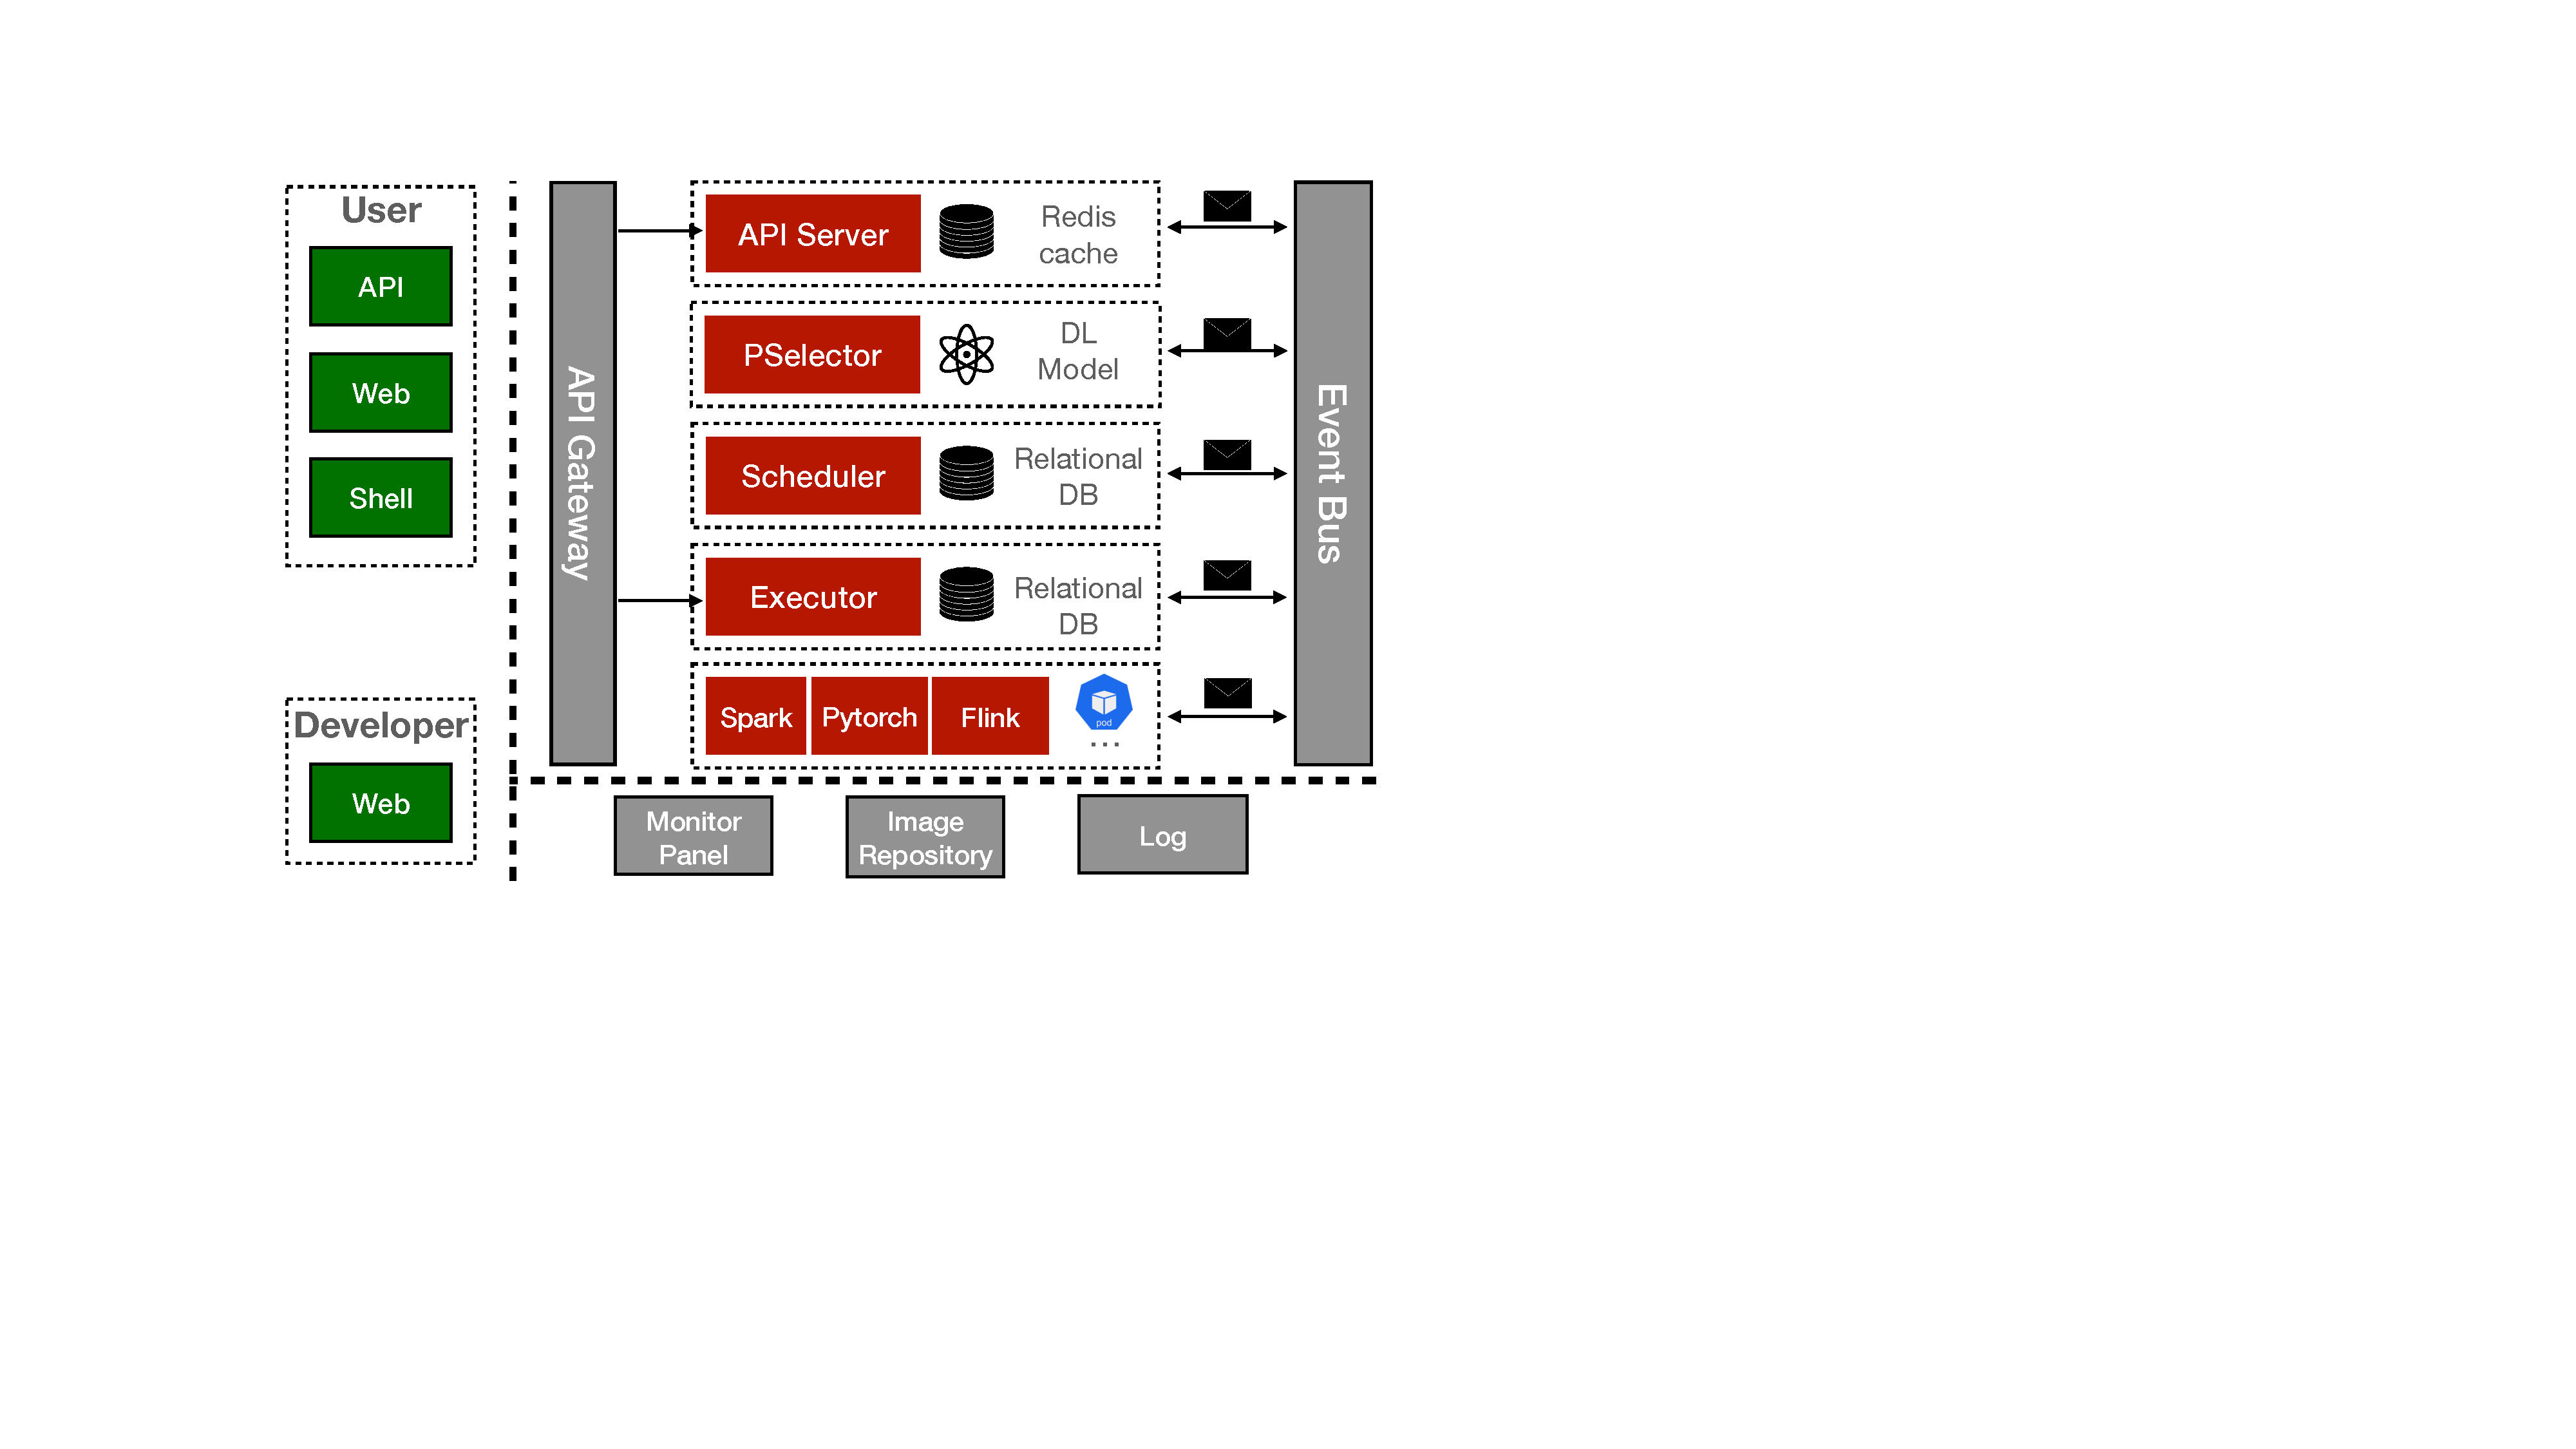
\includegraphics[width=0.8\linewidth]{figures/CLIC-arch-2.pdf}
    \caption{The architecture of CLIC}
    \label{fig:architecture}
\end{figure}


\textbf{Client}
Client offers a series logical operators and data models for building the workflow, and interfaces for task monitoring and controlment.
Since a real world workflow usually contains conditional branch (if-else clause) and iterations (while loop)
and the executing direction are determined dynamically[tensorflow, lara, rheem], 
the client also provides the flow controllers including SWITCH, NEXT ITERATION, and EXIT, to control the running direction of the workflow. 
For instance, the SWITCH controller has two output paths that are decided by the result of a given predicate.
The workflow or task control commands will be encapsulated and sent to the CLIC Service (API Gateway) by the client.
There are three forms of clients for user for different needs, that are API, Web, and Shell.

In addition, CLIC also provides developers with a series of interfaces for monitoring clusters, maintaining computing platforms, operators and other functions.

% Client 提供给用户一系列运算符和data model用于构建workflow;并提供用于任务监控和控制的接口;
% 用户提交的任务或控制命令经过 client 封装后会提交到 CLIC Services;
% 除此之外,CLIC 还为开发者提供了一系列接口用于监控集群、维护计算平台、运算符等功能。

\textbf{MicroServices}
Microservices enable flexibility where each module can be devleoped, tested and deployed independently. 
As shown in the figure, the server end contains four microservices and a global data store (GAS).
All the microservices interact with each other through the event bus in GAS.

The main microservices are as follows. 
a) API Server receives requests from clients and responds to it whenver the result is ready. 
For example, when receiving a task status lookup request, API Server publishs the event to the specific channel in the event bus and starts to listen. 
After the Executor microservice responds and API server receives the result ready event, it wraps the result with headers and responses to the client. 
b) PSelector takes a logical plan as input and outputs a physical plan with each operator being assigned with a platform. 
Inside the PSelector, it first encodes the operator to a feature vector and then utilizes a GNN model to predict platforms. 
The selecting details will be disscussed in Section 5.
After selecting the platform, the adjacent operators that belong to the same platform are packaged as a sub-task and then updates the specific field in GAS.
c) Scheduler specifies the number of a task's container instances and the targeted nodes to be deployed etc. according to the status of all resources maintained in GAS.
With the microservice architecture, different scheduling policies can be developed as independent microservices and deployed according to requirements of production systems.
% The resource status are periodically retreived from Executor and maintained in the GAS. 

\textbf{Executor}
Executor executes the tasks and monitors tasks and clusters.
It consists of a proxy program and a driver program. 
The proxy program 
1) accepts the task by listening to the event bus, 
2) communicates to the Kubernetes cluster for cluster running states, 
and 3) periodically reports the task status to GAS.
The driver program translates the task to the platform's job using platform API and submits it for execution.
The translation rule will be introduced in Section 4.2.


% The controlment includs instantiating, pausing, destroying the container and restarting jobs whenever it fails. 
% All the platform-related configuration files like container and network are declared in the form of YAML and managed by Helm [] charts and passed to the deployed platforms in execution. 

% These four core components are developed and deployed independently, making CLIC a flexible system with high availability.


\subsection{Operator Mapping and Management}
The Operations include the logical operator and flow controller. 
A logical operator represents a basic computational task such as data filtering or a K-Nearest-Neighbor(KNN) algorithm.
It is platform-independent and only describe the computational semantics like functionality, parameter list, input/output data format.
The implementation of a logical operator on a speicific platform is called as a physical operator.
There is a 1-N (N $\ge$ 1) mapping between a logical operator and physical operators, which means a logical operator can be implemented on multiple data processing platform.
A logical operator need to be transformed to a physical operator for execution, which will be discussed later.

Since a real world workflow usually contains conditional branch (if-else clause) and iterations (while loop)
and the executing direction are determined dynamically[tensorflow, lara, rheem], 
we introduce the flow controller such as SWITCH, NEXT-ITERATION to control the running direction of the workflow. 

CLIC offers Data Model & Operations.
Data Model :
% Since platforms may have different data models, e.g., table, matrix/vector and graph, CLIC provides a set of data model transformation operators that developers can directly use to convert data models.
% Besides that, a data model may have various data formats, such as a table can be row-based or column-based while the format a matrix can be block-partitioned or row-partitioned.
% Different computing paradigms require different data models.
% In order to support multiple paradigms, CLIC offers various data models, e.g. Table, Dictionary, Matrix/Vector and Graph.
% For a hybrid workflow that contains multiple paradigms, CLIC provides a set of model conversion operations to link two paradigms.

Operations:
% 前面提到过,logical -> physical 1 -> N

\textbf{Cloud-Native Task Deployment} 
Besides designing the cloud-native framework, CLIC decouples data processing platforms from the framework to facilitate extensible platform integration and independent deployment.
All physical operators of a platform are built in an image, thus each platform is developed and maintained independently.
To execute physical operators in one job, a platform image contains a proxy and a driver program.
The proxy program accepts the job submit and parse it to domain-specific-language (DSL). 
The driver program submits the DSL written job to the physical platform like Spark cluster, Tensorflow cluster, etc.


Moreover, one platform of different versions are kept as separate images to provide backward compatibility.

To mitigate expensive data transfer between operators, the input and output of an operator is an abstraction of the platform (e.g., RDD or numpy.array) or a specific data structure (int [] in C).
In this way, when adjacent tasks belong to the same platform, they can be merged and deployed as one job.
Instead, tasks of different platforms are launched as separate jobs and passes data through a file system.
After platform selection, each task in a workflow is assigned with an image of its corresponding platform.

To execute physical operators in one job, a platform image contains a driver program to drive the workflow execution. 
In the deployment of a job, Executor passes the operators information of the job to the driver program in the platform image. 
The driver program calls the specified data source operator to read data from the file system and transfers into the input abstraction and formats of operators, such as building an RDD. Then driver program interprets the workflow, calls the corresponding operators and passes data one by one. In the end, the driver program calls the data sink operator to serialize data and write to specified directory in the file system.
Overall, CLIC merges and deploys operators of the same platform as one task while automatically connecting adjacent platforms with automatic data transformation. 


% As shown in the figure, the CLIC server consists of a publish/subscribe mode event bus. 
% All the microservices interact with each other by publishing and subscribing to a specific channel in the event bus.


\subsection{Physical Operator}
mapping, management.

\subsection{Platform Selection}
%  CLIC first encodes the operators to vectors and then utilizes the Graph Convolutional Network(GCN) to solve this problem.
% 说到 there exists a best one,CLIC 会根据factor(可以直接说哪些factor) 自动选出最好的,就行了
% 其余的放在 sec.5 讲

% Each logical operator in the workflow need to be first transformed to a specific physical operator for execution.
% Although, a logical operator can have multiple available physical operators, there exists a best one, transforming to which can lead to the best overall performance. 

% 每个opt都要映射为physical 才行 。
% 有一个是best
% 找best需要取决于数据量、计算任务、硬件。

% For the flexibility of expanding the fast growing platforms, the GCN model is made adaptive to new platforms without retraining the model.
% Moreover, the model is designed as hardware-conscious to cope with the computing resource variations.

% To automatically select the best physical operator,
% CLIC first encodes the operators to vectors and then utilizes the Graph Convolutional Network(GCN) to solve this problem.



\subsection{Case Study}
We adopt sentiment classification as a case to demonstrate how CLIC works. It is a common nature language processing task that classifies documents based on the semantics. The data processing tasks mainly include data ETL (Extract, Transforming, Loading) and training of a classification model. The pseudo-code of a simple implementation is shown in Listing \ref{code:workflow}.

\begin{listing}[ht]
\begin{minted}[frame=lines,
framesep=2mm,
baselinestretch=1.2,
fontsize=\footnotesize,
linenos]{python}
source1 = read('BBC-News.txt’)
source2 = read('Hamlet.txt')
corpus = join(clean_source1, clean_source2)

word_embedding = toMatrix(clean_corpus, Word2Vec)
    
model = Model('LSTM')
train(model, word_embedding['train'])
topic = test(model, word_embedding['test'])
\end{minted}
\caption{Pseudo-code of sentiment classification in CLIC}
\label{code:workflow}
\end{listing}
The processing steps are as follows. 1) Based on logical operators, PlanBuilder builds the logical plan for the workflow. As shown in Figure \ref{fig:dag1}, the logical plan is a  DAG consists of five logical operators. 2) Optimizer applies optimizations on the logical plan. In this case, because the data volume of \textit{source2} is way lesser than source1, CLIC implicitly inserts a \textit{broadcast} operator to put \textit{source2}’s data on all nodes in order to reduce communication times. The optimized logical plan is shown in Figure \ref{fig:dag2}. 3) Logical operators are assigned to platforms with a GCN model. Figure \ref{fig:dag3} shows the potential platforms of each logical operator and marks the selected platforms with red triangles. Two platforms are selected in this case, where model training is placed on Pytorch while the rest operators are assigned to Spark. 4) The adjacent Spark operators and the PyTorch operator are grouped into two tasks as shown in Figure \ref{fig:dag4}, because merging adjacent operators of the same platform as one task can mitigate data transfer overheads. Then Scheduler chooses the corresponding container images for the two tasks and deploys them on the cloud subsequently. Note that, in the generation of the physical plan, PlanBuilder implicitly inserts a \textit{sink} operator in Spark to output the intermediate results and a \textit{source} operator in Pytorch to read Spark’s results.
